\chapter{Daftar Mata Kuliah, KRS, dan Penilaian}

\section{Transkrip}
\begin{center}

\includegraphics[page=1,width=0.97\textwidth,keepaspectratio]{\detokenize{assets/Transkrip Sementara Semester Gasal 2025-2026.pdf}}
\end{center}
\clearpage

\includepdf[
    pages=2-,
    frame=true,
    scale=0.8,
    pagecommand={\thispagestyle{fancy}}
]{\detokenize{assets/Transkrip Sementara Semester Gasal 2025-2026.pdf}}

\subsection{Daftar Mata Kuliah}
\begin{table}[htbp]
	\centering
	\small
	\begin{tabular}{|c|l|>{\raggedright\arraybackslash}p{8.7cm}|c|}
		\hline
		\textbf{No}                                             & \textbf{Kode MK} & \textbf{Nama MK/Kegiatan}                       & \textbf{SKS} \\
		\hline
		3                                                       & MII21-3011       & Internship: Pengembangan Fitur dan Modul Proyek & 4            \\
		\hline
		4                                                       & MII21-3015       & Internship: Pengujian Unit dan Modul Proyek     & 3            \\
		\hline
		5                                                       & MII21-4010       & Soft Skill: Kemampuan Berkomunikasi             & 2            \\
		\hline
		\multicolumn{3}{|r|}{\textbf{Jumlah SKS Kegiatan MBKM}} & \textbf{9}                                                                        \\
		\hline
	\end{tabular}
	\caption{Daftar Mata Kuliah Kegiatan MBKM}
	\label{tab:daftar_mk_mbkm}
\end{table}

\section{Formulir Penilaian Kinerja Mahasiswa Magang}
\clearpage
\refstepcounter{section}
\addcontentsline{toc}{section}{\protect\numberline{\thesection}Formulir Penilaian Kinerja Mahasiswa Magang MBKM}
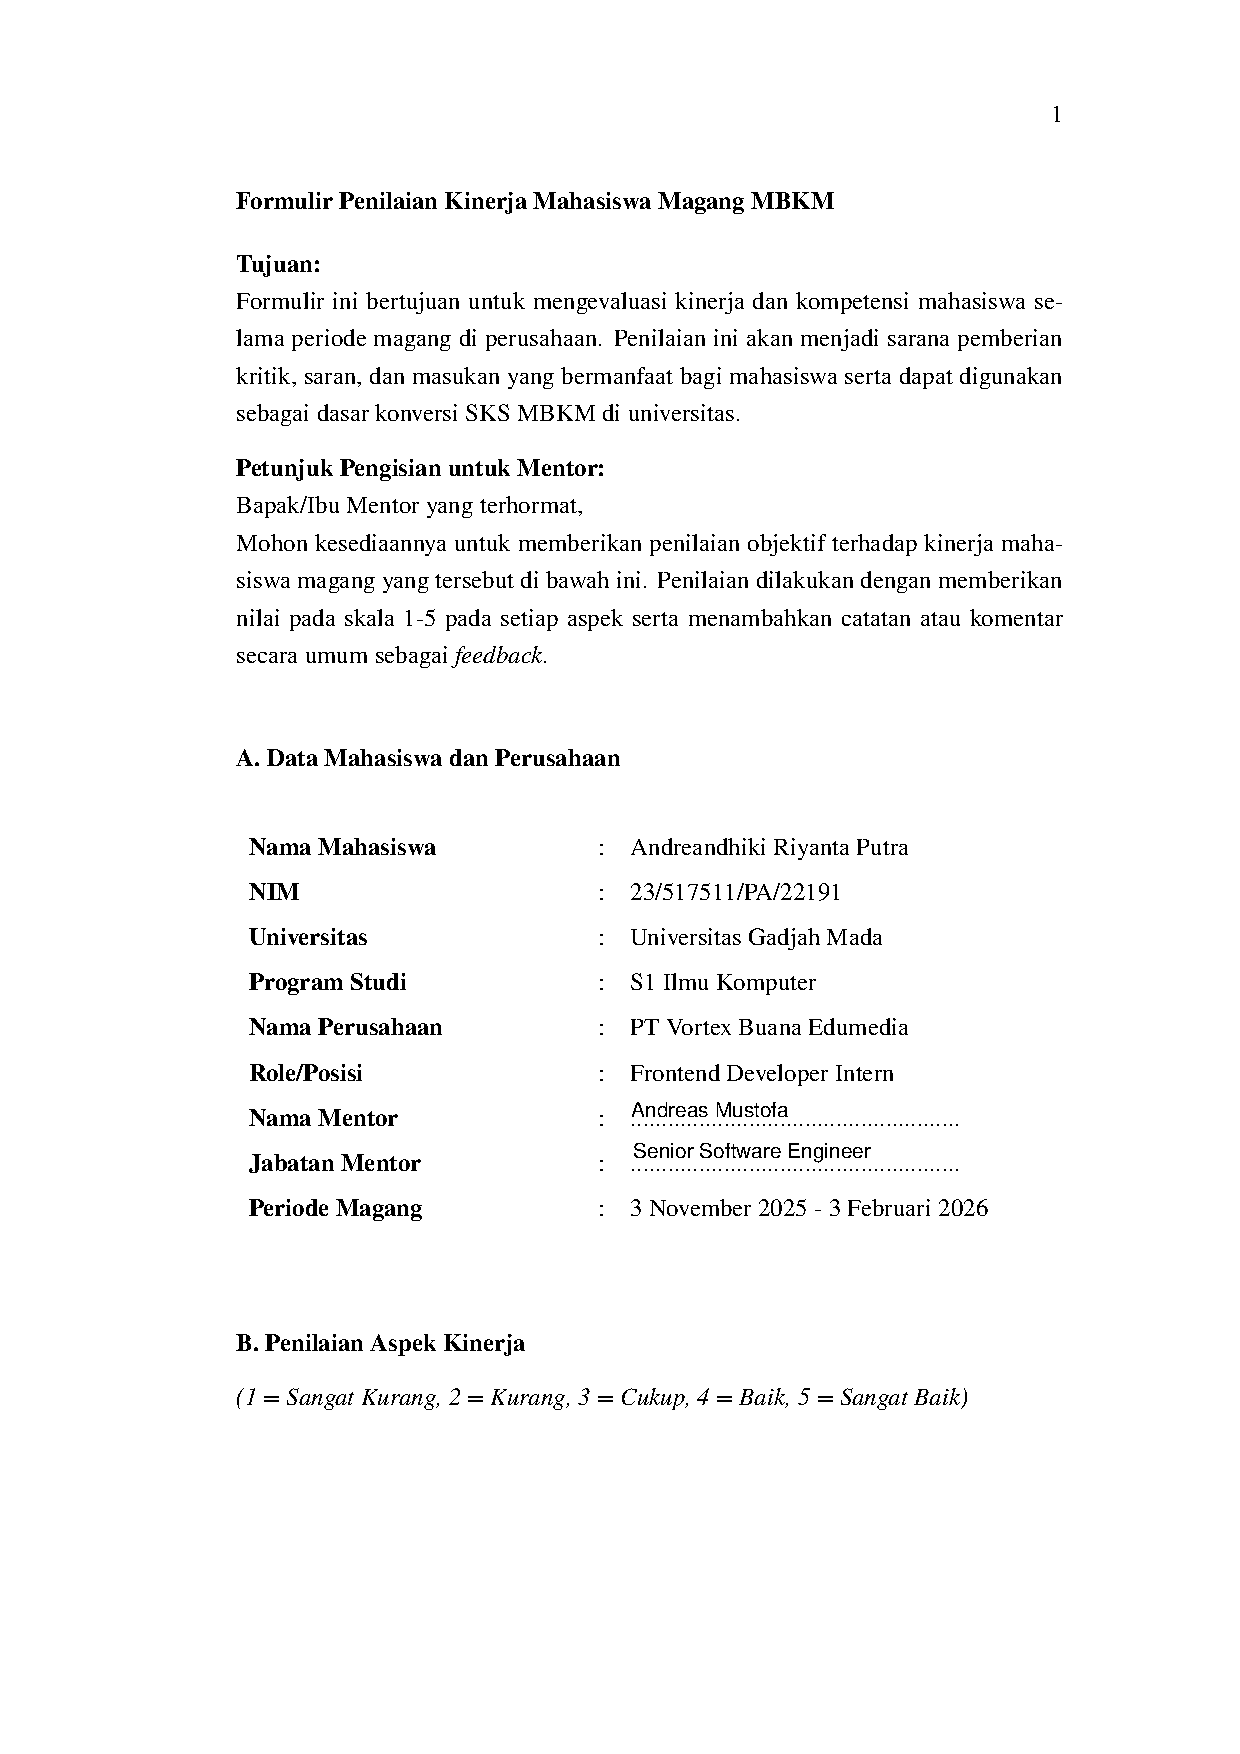
\includepdf[
	pages=-,
	frame=true,
	scale=0.8,
	pagecommand={\thispagestyle{fancy}}
]{assets/form_penilaian_mbkm_andreandhiki_riyanta_putra.pdf}

